\section{Infrastructure cloud transformation}
\label{sec:to-be}

The goal of Low Tech GmbH's cloud transformation is to modernize the existing infrastructure by transitioning to a scalable, secure, and highly available cloud environment. This will be achieved through the adoption of a hybrid cloud strategy leveraging private and colocated cloud solutions, and implementing a microservices architecture powered by Docker and Kubernetes. By embracing cloud-native technologies and open-source solutions, Low Tech GmbH aims to enhance system reliability, optimize operational efficiency, reduce costs, and enable future scalability while ensuring robust data security and compliance.

\section{Hybrid Cloud Solution for LowTech GmbH: Private and Colocated Infrastructure}

For LowTech GmbH, a \textbf{private and colocated hybrid cloud solution} offers an optimal balance between flexibility, control, scalability, and security. This hybrid infrastructure combines the benefits of a \textbf{private cloud} for sensitive applications and data with the advantages of \textbf{colocated hosting} for enhanced scalability and resource management. Such a solution aligns with LowTech GmbH’s goal to modernize its infrastructure while retaining control over critical systems and data, with a view to migrating to a \textbf{public cloud} in the future.

\subsection{Private Cloud Infrastructure for Sensitive Applications}

LowTech GmbH’s sensitive applications, such as finance systems, HR, and payroll data, require stringent compliance with privacy regulations and data security policies. These systems will reside within a \textbf{private cloud} environment, either hosted on-premises or in a private data center. The private cloud offers LowTech GmbH full control over infrastructure and data management, ensuring compliance with regulations like \textbf{GDPR} or \textbf{HIPAA}.

To support LowTech GmbH’s ongoing modernization efforts, the private cloud will use advanced \textbf{virtualization technologies} (such as \textbf{VMware} or \textbf{OpenStack}) and \textbf{Kubernetes} for container orchestration. Kubernetes will allow the company to efficiently deploy, manage, and scale \textbf{microservices-based applications}. This approach modernizes existing legacy systems by breaking them into smaller, independently deployable services, enhancing flexibility, performance, and maintainability.

\subsection{Colocated Hosting for Scalability and Flexibility}

In the context of \textbf{colocated hosting}, LowTech GmbH will deploy its physical servers in a \textbf{third-party data center} while retaining control over the hardware. This solution enables the company to scale its infrastructure efficiently, ensuring that hardware needs for high-demand workloads (such as the \textbf{Sales} and \textbf{Operations} departments) are met without the burden of managing an internal data center. Colocated hosting also improves resource allocation, as it provides more flexibility than a purely on-premises solution, allowing LowTech GmbH to manage infrastructure without significant upfront capital investments.

By combining both private cloud and colocated hosting, LowTech GmbH can expand infrastructure capacity on demand. This hybrid model provides \textbf{high-performance computing} for specialized applications while leveraging the physical security and networking benefits of a colocated data center.

\subsection{Hybrid Cloud Architecture: Integration of Private and Colocated Infrastructure}

In the \textbf{hybrid architecture}, the private cloud will host \textbf{core applications} and sensitive data, while colocated servers will manage resource-intensive or overflow workloads. Key features of this hybrid solution include:

\begin{itemize}
    \item \textbf{Infrastructure as a Service (IaaS)}: Both the private cloud and colocated hosting will use an IaaS model, enabling LowTech GmbH to provision virtualized servers dynamically. The private cloud will handle core operations such as finance and CRM, while the colocated infrastructure will support high-demand applications or data overflow.
    
    \item \textbf{Microservice Architecture}: LowTech GmbH’s legacy applications will be decomposed into microservices, enhancing scalability and flexibility. For example, the \textbf{CRM} and \textbf{Order Management} applications will be broken down into independent services, deployed across both the private cloud and colocated infrastructure as per performance and security requirements.
    
    \item \textbf{Containerization with Kubernetes}: Both the private and colocated environments will use \textbf{Docker containers} orchestrated by \textbf{Kubernetes}. Containers enable efficient, portable deployment of services, and Kubernetes ensures the seamless management of microservices across both infrastructures.
    
    \item \textbf{Data Integration}: To maintain seamless data flow between the private cloud and colocated infrastructure, tools like \textbf{APIs} and \textbf{service meshes} (e.g., \textbf{Istio}) will be employed. This ensures that data consistency and communication are maintained across both environments, allowing LowTech GmbH to integrate legacy systems with modern cloud-native applications.
    
    \item \textbf{Disaster Recovery and Business Continuity}: The colocated infrastructure will play a critical role in \textbf{disaster recovery} (DR). It provides a geographically redundant backup for the private cloud, ensuring that critical applications and data remain available even in case of infrastructure failure. LowTech GmbH will also leverage \textbf{backup solutions} to protect important business data, further securing the organization’s business continuity.
\end{itemize}

\subsection{Security and Compliance for Sensitive Data}

A hybrid cloud solution allows LowTech GmbH to retain tight control over sensitive data, addressing security and compliance concerns while benefiting from the flexibility of cloud technology:

\begin{itemize}
    \item \textbf{Data Encryption}: Encryption will be applied both in-transit and at-rest to protect data. Sensitive financial and HR information will remain within the private cloud or colocated servers, with strict controls to prevent unauthorized access.
    
    \item \textbf{Access Control}: The private cloud and colocated hosting will implement \textbf{role-based access control (RBAC)} and \textbf{identity and access management (IAM)} solutions, ensuring that only authorized users have access to sensitive applications and data.
    
    \item \textbf{Network Security}: Both private and colocated infrastructures will utilize \textbf{virtual private networks (VPNs)}, \textbf{firewalls}, and \textbf{intrusion detection systems (IDS)} to safeguard against unauthorized access, ensuring the security of LowTech GmbH’s critical systems.
\end{itemize}

\subsection{Scalability and Flexibility in the Hybrid Cloud Model}

The hybrid cloud solution provides LowTech GmbH with the flexibility to scale its infrastructure based on business needs:

\begin{itemize}
    \item \textbf{Scalability}: The private cloud will handle core operations and sensitive applications, while the colocated infrastructure will scale to meet fluctuating demands, particularly for workloads in \textbf{Sales}, \textbf{Operations}, and other high-performance departments. By colocating servers, LowTech GmbH can easily increase its capacity without significant upfront investments.
    
    \item \textbf{Flexibility}: The hybrid solution allows LowTech GmbH to optimize its workloads based on performance, security, and regulatory requirements. For instance, sensitive data can be maintained in the private cloud or colocated servers, while less critical workloads can be offloaded to the public cloud as needed.
\end{itemize}

\subsection{Future Migration to Public Cloud}

The hybrid cloud infrastructure will serve as an intermediate step towards a full \textbf{public cloud migration}. As LowTech GmbH moves to a public cloud in the future, the hybrid architecture will provide the necessary flexibility for gradual adoption. By leveraging \textbf{containers} and \textbf{microservices}, applications will be made portable and cloud-agnostic, allowing LowTech GmbH to migrate workloads to public cloud platforms like \textbf{AWS}, \textbf{Azure}, or \textbf{Google Cloud Platform (GCP)}. This approach ensures that LowTech GmbH maintains control over sensitive data during the transition while still benefiting from the scalability and cost-efficiency of the public cloud.




\begin{figure}[H]
\centering
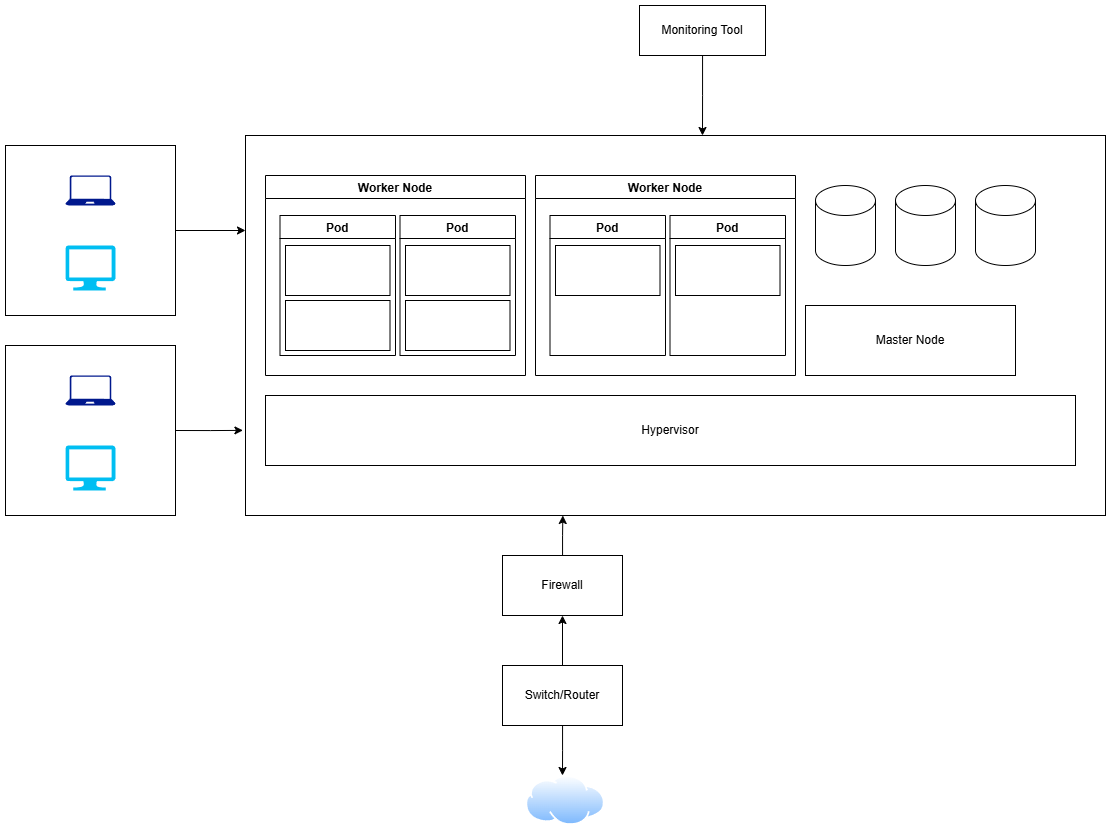
\includegraphics[width=1\textwidth]{Images/K8_cluster} 
\caption{Kubernetes Cluster}
\label{fig:vite}
\end{figure}


\section{Hardware and Software Components for New Infrastructure}

\subsection*{Hardware Components}
\begin{itemize}
    \item \textbf{Servers:}
    \begin{itemize}
        \item Virtualized Servers (for Kubernetes Nodes)
        \item Application Servers (for microservices deployment)
        \item Storage Servers (for data storage needs)
        \item Web Servers (for web application hosting)
    \end{itemize}
    \item \textbf{Networking Equipment:}
    \begin{itemize}
        \item Switches (for intra-data center communication)
        \item Routers (for external connectivity)
        \item Firewalls (for network security)
        \item Load Balancers (for traffic distribution across services)
    \end{itemize}
    \item \textbf{Backup Devices:}
    \begin{itemize}
        \item Backup Servers (for storing backups of applications and databases)
    \end{itemize}
    \item \textbf{Storage:}
    \begin{itemize}
        \item SSD Storage (for high-performance applications)
        \item HDD Storage (for archival or less demanding workloads)
        \item Network Attached Storage (NAS) (for shared access and backups)
    \end{itemize}
    \item \textbf{Colocated Data Center Infrastructure:}
    \begin{itemize}
        \item Colocated Racks (for housing physical servers in third-party data centers)
        \item Cooling Systems (for maintaining optimal operating conditions)
        \item Power Supply Units (UPS) (for ensuring uninterruptible power supply)
    \end{itemize}
\end{itemize}

\subsection{Software Components}
\begin{itemize}
    \item \textbf{Operating Systems:}
    \begin{itemize}
        \item Linux (e.g., Ubuntu, CentOS, RedHat - for running Kubernetes nodes and containers)
    \end{itemize}
    \item \textbf{Virtualization and Containerization:}
    \begin{itemize}
        \item Docker (for containerizing microservices and applications)
        \item Kubernetes (for container orchestration and microservices management)
        \item OpenStack (for managing private cloud infrastructure)
    \end{itemize}
    \item \textbf{Networking and Security:}
    \begin{itemize}
        \item pfSense (for network security, firewalls, and VPN setup)
        \item Intrusion Detection Systems (IDS) (for network security monitoring)
        \item VPN Software (for secure remote access)
    \end{itemize}
    \item \textbf{Backup and Disaster Recovery:}
    \begin{itemize}
        \item Backup Software (e.g., Veeam, Bacula - for application and server backups)
        \item Cloud Backup Solutions (for offsite backup storage)
    \end{itemize}
    \item \textbf{Monitoring and Logging:}
    \begin{itemize}
        \item Prometheus (for system and application monitoring)
        \item Grafana (for visualizing metrics and performance data)
        \item ELK Stack (Elasticsearch, Logstash, Kibana - for centralized logging and analytics)
    \end{itemize}
    \item \textbf{Database Management Systems:}
    \begin{itemize}
        \item MySQL (for relational data storage)
        \item PostgreSQL (for relational data storage with advanced features)
        \item MongoDB (for NoSQL data storage)
    \end{itemize}
    \item \textbf{Cloud Management:}
    \begin{itemize}
        \item OpenStack (for managing the private cloud infrastructure)
        \item Kubernetes (for managing containerized applications and microservices across clusters)
    \end{itemize}
\end{itemize}


\section{Energy Consumption and Cost Considerations}

As LowTech GmbH transitions to a hybrid cloud infrastructure, energy consumption and cost efficiency are critical factors. The new infrastructure focuses on reducing both server and client energy demands while maintaining performance and scalability.

\subsection{Servers}

In a Kubernetes-based environment, energy consumption depends on hardware efficiency. To optimize power usage:
\begin{itemize}
    \item \textbf{Energy-efficient hardware}: Using modern servers, such as ARM-based processors, reduces energy consumption.
    \item \textbf{Dynamic resource allocation}: Kubernetes scales workloads based on demand, minimizing idle power usage.
    \item \textbf{Data center efficiency}: Colocated data centers provide optimized cooling and power management, reducing overall energy costs.
\end{itemize}

These measures help keep server-related electricity costs low while maintaining performance.

\subsection{Clients}

Switching from traditional desktops to energy-efficient mini PCs and laptops can significantly reduce electricity consumption:
\begin{itemize}
    \item \textbf{Mini PCs}: These devices consume less than 30W (often under 15W), are priced under €500, and are more than capable of running cloud applications.
    \item \textbf{Laptops}: With power usage ranging from 15W to 50W, laptops are efficient for cloud-based tasks.
\end{itemize}

By adopting mini PCs and laptops, LowTech GmbH can reduce the energy consumption of client devices, leading to lower electricity costs and environmental impact.

\subsection{Cost Summary}

By utilizing energy-efficient server hardware, Kubernetes for dynamic resource allocation, and switching to mini PCs and laptops for clients, LowTech GmbH will reduce operational costs. These energy-saving strategies will ensure that the company maintains a balance between cost-effectiveness, scalability, and environmental sustainability.


